\documentclass{article}

\usepackage{graphicx}
\usepackage{tikz}
\usepackage{tikzsymbols}
\usetikzlibrary{calc,patterns,shapes.geometric}
\pagestyle{empty}
\usepackage[margin=0pt]{geometry}
\geometry{papersize={14in,12in}}

\def\centerarc[#1](#2)(#3:#4:#5){\draw[#1] ($(#2)+({#5*cos(#3)},{#5*sin(#3)})$) arc (#3:#4:#5);}

\begin{document}
	\begin{figure}
		\centering
		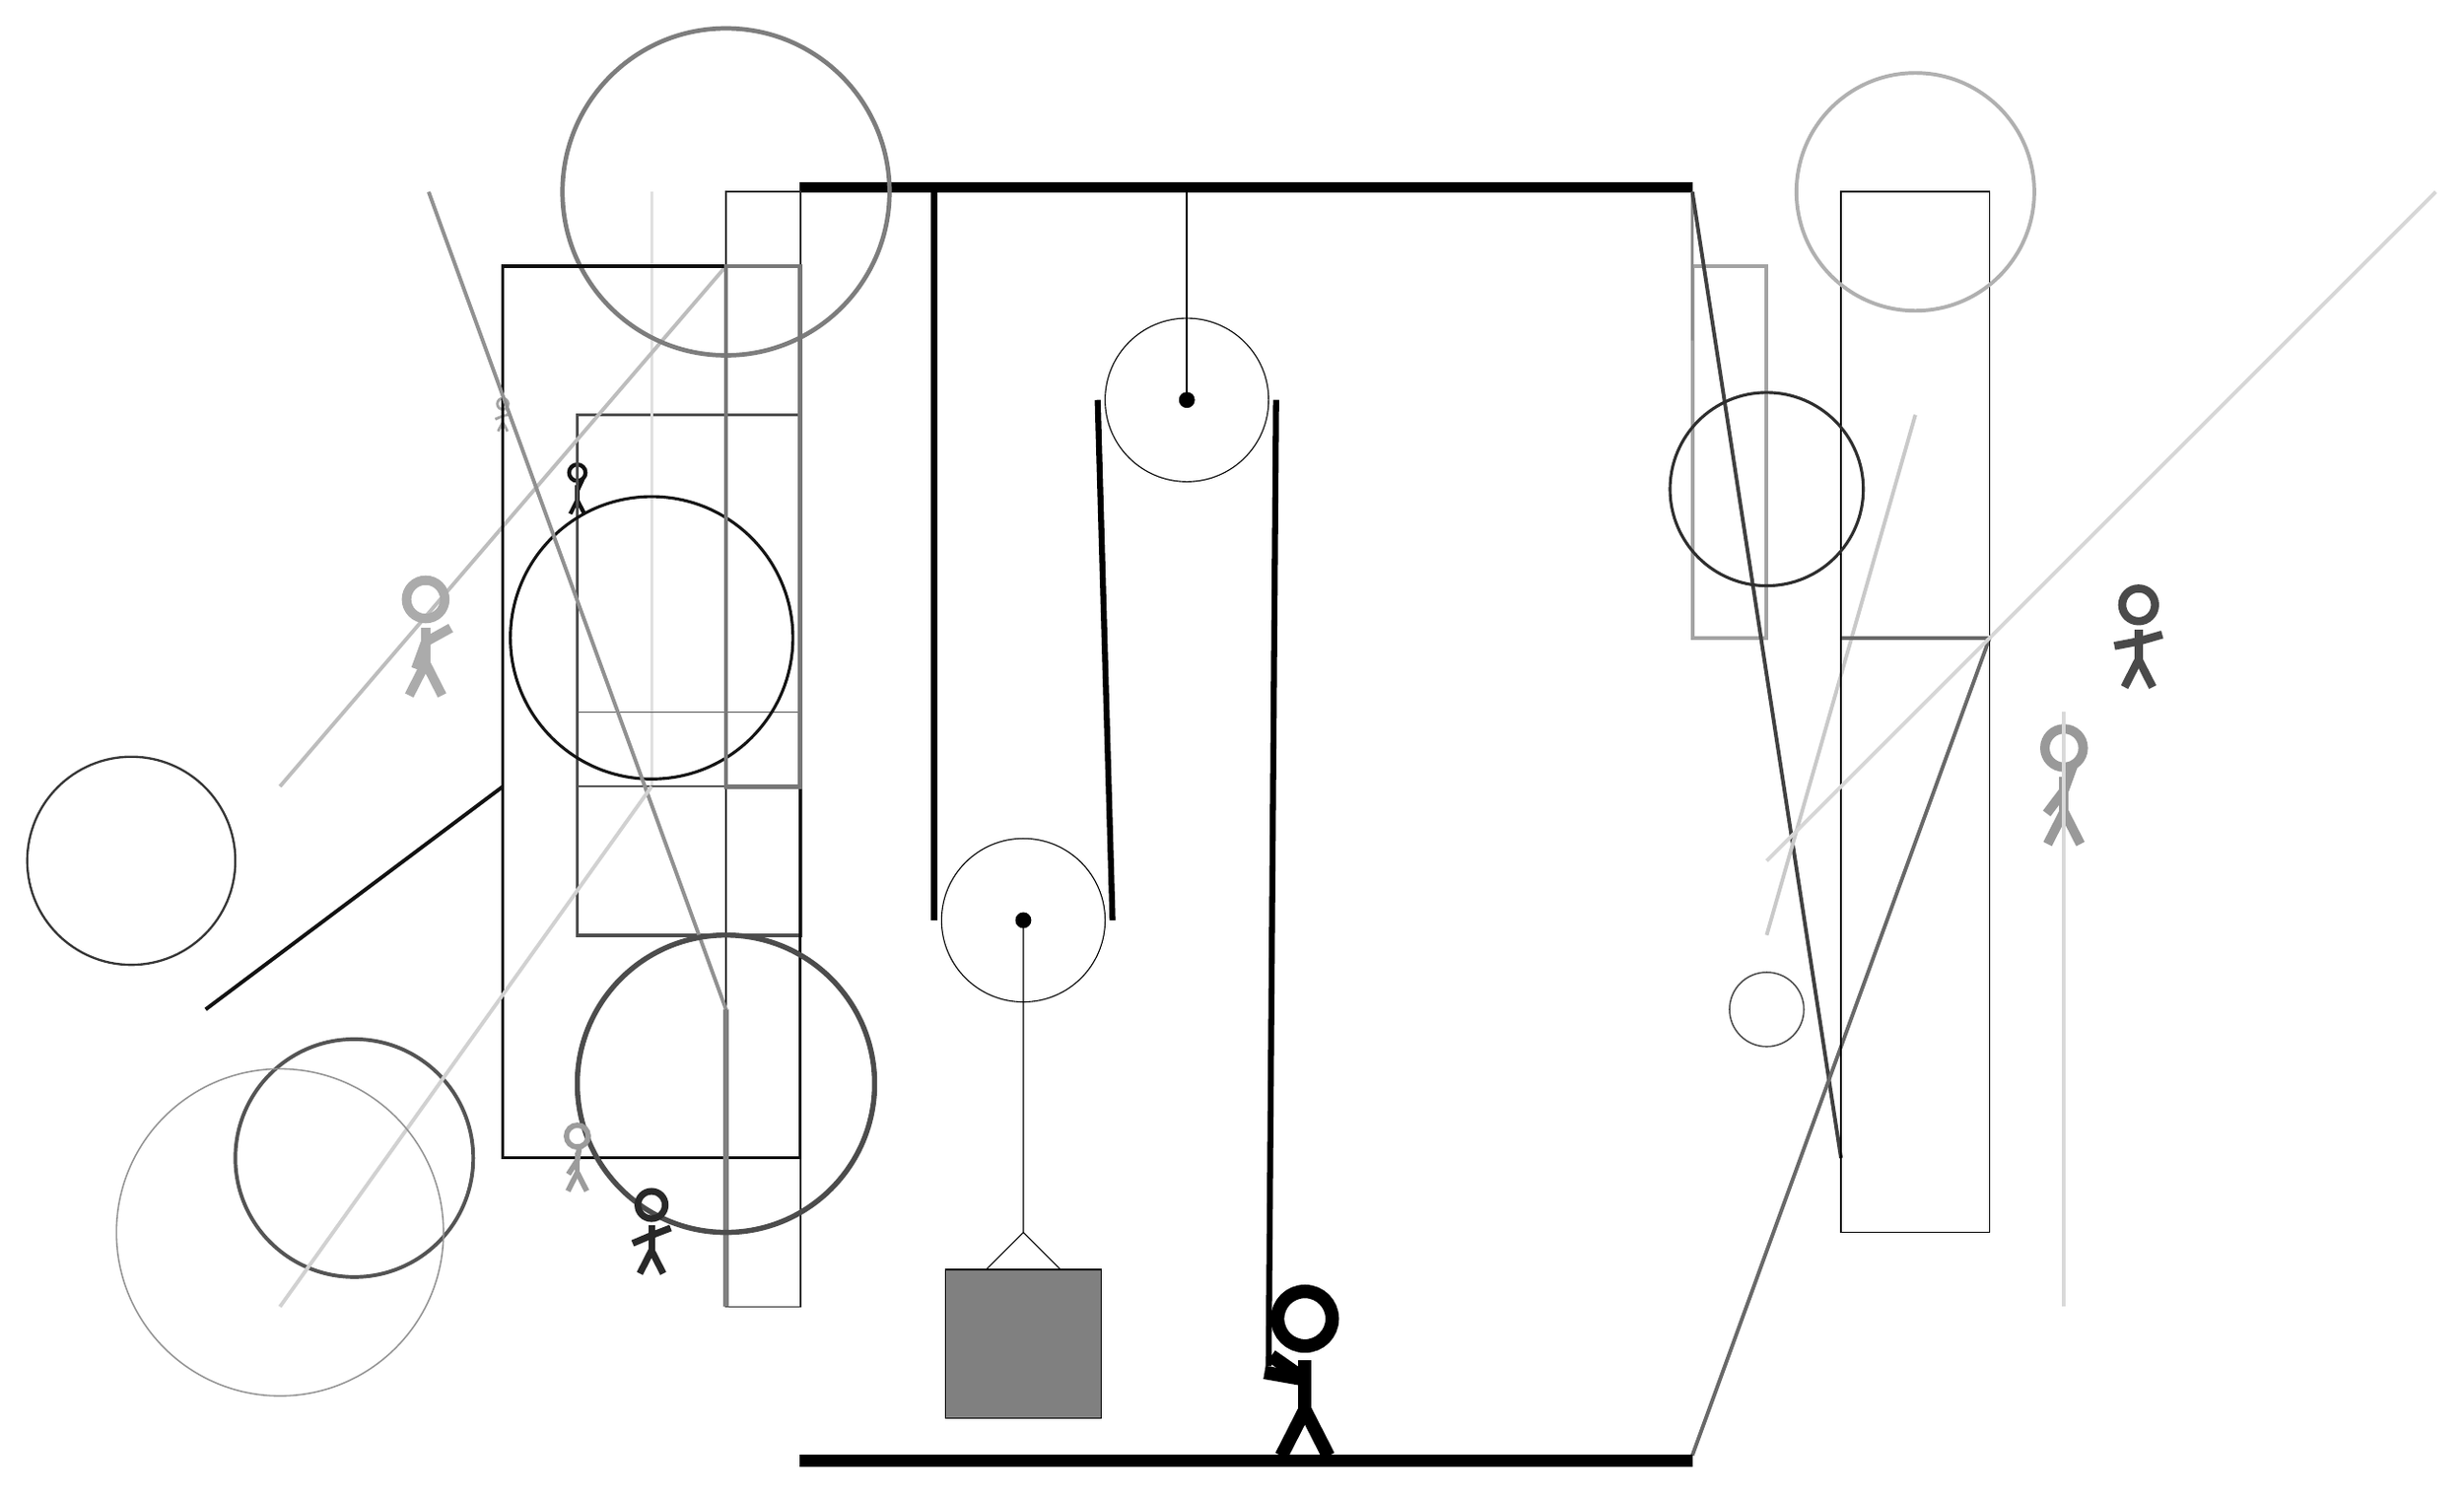
\begin{tikzpicture}
			%%%%% START %%%%%
			
			\draw[fill=black] (-2, 14) rectangle (10, 14.125);
			
			\draw (3.2, 11.2) circle (1.1);
			\draw[fill=black] (3.2, 11.2) circle (0.1);
			\draw[thick] (3.2, 11.2) -- (3.2, 14);
			
			\draw (1, 4.2) circle (1.1);
			\draw[fill=black] (1, 4.2) circle (0.1);
			
			\draw[line width=0.2mm, color=black!84] (-2, -1) rectangle (-3, 14);
			
			\node[line width=0.5mm, color=black!93] at (-5, 10) {\Strichmaxerl[3][88][65]};
			\draw[line width=0.5mm, color=black!36] (11, 8) rectangle (10, 13);
			\draw[line width=0.5mm, color=black!69] (-2, 11) rectangle (-5, 4);
			\draw[line width=0.4mm, color=black!45] (10, 14) rectangle (10, 12);
			\draw[line width=0.4mm, color=black!12] (-4, 6) rectangle (-4, 14);
			\draw[line width=0.5mm, color=black!75](12, 1) -- (10, 14);
			\node[line width=0.2mm, color=black!36] at (-6, 11) {\Strichmaxerl[2][23][14]};
			\draw[line width=0.5mm, color=black!26](-3, 13) -- (-9, 6);
			
			\draw [line width=0.6mm, color=black!51](-3, 14) circle (2.2);
			
			\draw[line width=0.5mm, color=black!21](13, 11) -- (11, 4);
			\node[line width=0.4mm, color=black!40] at (15, 6) {\Strichmaxerl[7][53][70]};
			\draw[line width=0.4mm, color=black!94] (-2, 1) rectangle (-6, 13);
			
			\draw[line width=0.5mm, color=black!59](14, 8) -- (10, -3);
			\draw[line width=0.5mm, color=black!59](12, 8) -- (14, 8);
			\draw [line width=0.2mm, color=black!70](11, 3) circle (0.5);
			
			\draw[line width=0.2mm, color=black!68] (-2, 6) rectangle (-5, 7);
			\draw[line width=0.7mm, color=black!50] (-3, -1) rectangle (-3, 3);
			\draw[line width=0.2mm, color=black!99] (12, 14) rectangle (14, 0);
			
			\draw [line width=0.3mm, color=black!79](-11, 5) circle (1.4);
			\node[line width=0.3mm, color=black!71] at (16, 8) {\Strichmaxerl[6][11][16]};
			
			\draw [line width=0.5mm, color=black!31](13, 14) circle (1.6);
			\draw[line width=0.5mm, color=black!16](11, 5) -- (20, 14);
			\draw [line width=0.5mm, color=black!67](-8, 1) circle (1.6);
			\draw [line width=0.4mm, color=black!92](-4, 8) circle (1.9);
			
			\draw [line width=0.4mm, color=black!82](11, 10) circle (1.3);
			\draw[line width=0.5mm, color=black!43](-7, 14) -- (-3, 3);
			\draw[line width=0.5mm, color=black!18](-4, 6) -- (-9, -1);
			\draw [line width=0.7mm, color=black!70](-3, 2) circle (2.0);
			\node[line width=0.5mm, color=black!33] at (-7, 8) {\Strichmaxerl[7][70][29]};
			\node[line width=0.4mm, color=black!39] at (-5, 1) {\Strichmaxerl[4][57][81]};
			
			\draw[line width=0.6mm, color=black!53] (-3, 13) rectangle (-2, 6);
			\draw [line width=0.2mm, color=black!42](-9, 0) circle (2.2);
			
			\node[line width=0.5mm, color=black!84] at (-4, 0) {\Strichmaxerl[5][23][21]};
			\draw[line width=0.5mm, color=black!93](-6, 6) -- (-10, 3);
			\draw[line width=0.5mm, color=black!15](15, 7) -- (15, -1);
			
			\draw (1, 4.2) -- (1, 0) -- (0.5, -0.5);
			\draw (1, 0) -- (1.5, -0.5);
			\draw[fill=black!50] (-0.05, -0.5) rectangle (2.05, -2.5);
			
			\draw[line width=0.8mm] (-0.2, 14) -- (-0.2, 4.2);
			\centerarc[line width=0.8mm](1, 4.2)(180:360:1.2000000000000002);
			\draw[line width=0.8mm](2.2, 4.2) -- (2.0, 11.2);
			\centerarc[line width=0.8mm](3.2, 11.2)(0:180:1.2000000000000002);
			\draw[line width=0.8mm](4.4, 11.2) -- (4.3, -1.8);
			
			\node at (4.7, -1.9) {\Strichmaxerl[10][-35][170]};
			
			\draw[fill=black] (-2, -3) rectangle (10, -3.15);
			
			%%%%% END %%%%%
		\end{tikzpicture}
	\end{figure}	
\end{document}